\chapter{Generación exhaustiva acotada basada en la API}
\label{cap:beapi}

En adelante, se presenta la técnica desarrollada llamada BEAPI, que tiene como
objetivo realizar la generación exhaustiva acotada (\emph{Bounded Exhaustive Generation}) 
de objetos usando los métodos de la API del módulo bajo test. 
La generación exhaustiva acotada es un enfoque de generación de tests que
consiste en generar todas las posibles entradas para el software bajo test con
dominios de datos acotados (usualmente pequeños). 
La mayor ventaja de la generación exhaustiva acotada es un enfoque efectivo para
revelar fallas en el software \cite{Marinov01,Khurshid01,Boyapati02,Sullivan04}.

Los enfoques existentes de generación exhaustiva acotada requieren una
especificación precisa y formal de las propiedades que deben satisfacer las
entradas del software bajo test \cite{Boyapati02,KhKhurshid01,Ponzio16Ponzio:2016,Rosner14}. 
Esta especificación comúnmente se llama \emph{repOK} (define las propiedades que
satisface la representación de las entradas) y debe ser brindada por el usuario \cite{Boyapati02,Khurshid01,Ponzio16Ponzio:2016,Rosner14}.
En este capítulo, introduciremos BEAPI, un enfoque eficiente que genera un
conjunto exhaustivo acotado de objetos realizando únicamente llamadas a la API
de un módulo. Al utilizar la API para construir objetos, BEAPI no requiere 
un \emph{repOK} como las técnicas existentes. 
Además, BEAPI incorpora optimizaciones novedosas en la generación de tests, que
mejoran significativamente su rendimiento, y son claves para realizar la generación exhaustiva acotada de manera eficiente. 

Este capítulo está organizado de la siguiente manera: en la Sección \ref{sec:motivating-example}, 
se presenta un ejemplo que ilustra el problema que se aborda con la técnica propuesta. 
La Sección \ref{sec:beapi-overview} presenta un panorama general de 
BEAPI. La Sección \ref{sec:scope} describe la definición del scope para la
técnica, y \ref{sec:defensiveProgramming} aborda como BEAPI evita construir
objetos inválidos si la API se programa de manera defensiva \cite{Liskov00}.
Luego, en las Secciones \ref{sec:stateMatching} y
 \ref{sec:buildersOptimization} se describen las optimizaciones implementadas en
 BEAPI, que son claves para mejorar su eficiencia, y le permiten a BEAPI 
lograr un rendimiento comparable al de las técnicas basadas en especificaciones
(como \emph{Korat}\cite{Boyapati02}). Finalmente, en la Sección 
\ref{sec:beapiTechnique} se presenta un pseudocódigo del algoritmo de BEAPI.


\section[Motivación]{Motivación}
\label{sec:motivating-example}


\begin{figure}[!thb]
\begin{lstlisting}
public boolean repOK() {
    if (this.header == null) return false;
    // Missing constraint: the value of the sentinel node must be null  
    // if (this.header.value != null) return false;
    if (this.header.next == null) return false;
    if (this.header.previous == null) return false;
    if (this.cacheSize > this.maximumCacheSize) return false;
    if (this.size < 0) return false;
    int cyclicSize = 0;
    LinkedListNode n = this.header;
    do {
        cyclicSize++;
        if (n.previous == null) return false;
        if (n.previous.next != n) return false;
        if (n.next == null) return false;
        if (n.next.previous != n) return false;
        if (n != null) n = n.next;
    } while (n != this.header && n != null);
    if (n == null) return false;
    if (this.size != cyclicSize - 1) return false;
    int acyclicSize = 0;
    LinkedListNode m = this.firstCachedNode;
    Set visited = new HashSet();
    visited.add(this.firstCachedNode);
    while (m != null) {
        acyclicSize++;
        if (m.previous != null) return false;
        // Missing constraint: the value of cache nodes must be null
        // if (m.value != null) return false;
        m = m.next;
        if (!visited.add(m)) return false;
    }
    if (this.cacheSize != acyclicSize) return false;
    return true;
}
\end{lstlisting}
\caption{\texttt{repOK} de \texttt{NodeCachingLinkedList} tomado del benchmark de \textsf{ROOPS}}
\label{fig:NCL-repOK}
\end{figure}
Las herramientas de generación exhaustiva acotada existentes, como \emph{Korat},
requieren de una especificación formal para poder distinguir las entradas
que válidas para el software bajo test de las inválidas (y descartar estas
últimas durante la generación).
En el caso de Korat, esta especificación se define mediante 
un método booleano en el mismo lenguaje de programación (Java), que toma como
parámetro una estructura y devuelve
\texttt{true} si y solo si la estructura satisface las propiedades deseadas.
Cuando se trata de implementaciones de estructuras de datos (un caso típico de
aplicación de la generación exhaustiva acotada), la especificación describe las
propiedades que debe satisfacer la representación de la estructura, por lo que 
el método que define la especificación usualmente se denomina \emph{repOK}~\cite{Boyapati02}. 

Para ilustrar las dificultades que implica escribir estas especificaciones de
forma precisa para el usuario de la herramienta, consideramos el método 
\emph{repOK} de la clase \texttt{NodeCachingLinkedList} (NCL) de Apache, que se
muestra en la Figura~\ref{fig:NCL-repOK}. 
Este ejemplo proviene del benchmark \emph{ROOPS}, que ha sido ampliamente
utilizado para evaluar herramientas automáticas de testing/análisis de software 
\cite{Pasareanu:2010,Rosner15,Galeotti:2010,galeotti2020,Boyapati02,Khurshid01}.

Como se explicó en el Capítulo~\ref{cap:builders}, NCL posee una lista
principal, implementada usando una lista circular doblemente enlazada, 
y una lista auxiliar simplemente enlazada que actúa como caché de nodos
previamente eliminados de la lista principal. Esta caché permite reutilizar 
nodos eliminados, evitando la sobrecarga de recolección de basura en aplicaciones con frecuentes inserciones y eliminaciones.

El método \texttt{repOK} verifica la validez estructural de una instancia de
NCL. Sin embargo, como se muestra en la Figura~\ref{fig:NCL-repOK}, el
autor del código en ROOPS olvidó describir algunas restricciones que deben
cumplir las instancias de NCL. Más específicamente, el autor omitió las
restricciones que indican que: el nodo ficticio de la lista principal debe tener el
valor \texttt{null} (líneas 3 y 4), y que los nodos de la caché no deben 
contener datos (líneas 28 y 29)). Como se discute más adelante, la omisión de estas 
condiciones conduce a la generación de una gran cantidad de estructuras
inválidas por parte de Korat.

\begin{figure}[p]
    \centering
    \begin{subfigure}[b]{\textwidth}
        \centering
        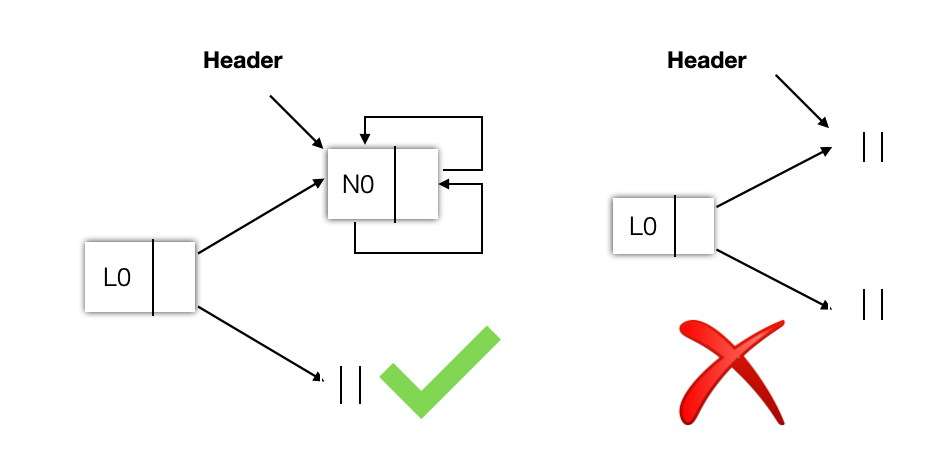
\includegraphics[width=0.8\textwidth]{images/repOK1.jpg}
        \caption{Ejemplo de una instancia válida y otra inválida debido a la
            falta de un nodo ficticio en la lista principal.}
        \label{fig:repOKa}
    \end{subfigure}

    \vspace{10pt}
    \begin{subfigure}[b]{\textwidth}
        \centering
        \includegraphics[width=0.8\textwidth]{images/repOK2.jpg}
        \caption{Ejemplo de una instancia válida y otra inválida debido a la
            ciclicidad de la lista principal.}
        \label{fig:repOKb}
    \end{subfigure}

    \vspace{10pt}

    \begin{subfigure}[b]{\textwidth}
        \centering
        \includegraphics[width=0.8\textwidth]{images/repOK3.jpg}
        \caption{Ejemplo de una instancia válida y otra inválida debido a la
            aciclicidad de la lista caché.}
        \label{fig:repOKc}
    \end{subfigure}

    \caption{Ejemplos de instancias de \texttt{NodeCachingLinkedList}.}
    \label{fig:repOK}
\end{figure}


En la Figura~\ref{fig:repOK} se muestran ejemplos de instancias válidas e inválidas, lo cual facilita entender visualmente las propiedades que deben estar reflejadas en la especificación.

Las líneas 2 a 10 del método \texttt{repOK} se centran en la verificación de aspectos estructurales básicos. Se asegura la existencia del 
nodo ficticio, y que debe estar correctamente conectado (se omite que debe contener el valor
\texttt{null}). 
En el ejemplo de la Figura~\ref{fig:repOKa}, la instancia de la izquierda es
válida; la de la derecha es inválida porque no posee un nodo ficticio, lo cual
es detectado por la condición de la línea 2.

Las líneas 9 a 20 validan que la lista principal sea circular y doblemente enlazada. Esto implica que el recorrido a partir 
del nodo ficticio debe eventualmente volver a él, y que cada nodo debe tener enlaces consistentes hacia su anterior y su 
siguiente. En otras palabras, si avanzamos a través de la lista desde el primer elemento, llegaremos eventualmente al
último elemento y luego volveremos al primer elemento. Además, se asegura que la cantidad de nodos visitados coincida con el valor del campo \texttt{size}.

En la Figura~\ref{fig:repOKb} se pueden observar ejemplos de instancias que satisfacen o no esta sección de restricciones del método.
La instancia de la izquierda muestra una lista principal correctamente construida, mientras que la instancia de la derecha presenta el error de que la lista principal no es circular.  
En esta instancia, el campo \emph{next} del nodo final no apunta nuevamente al nodo ficticio, lo que rompe la propiedad de circularidad de la estructura.  
Esta restricción está controlada en las líneas 15 y 16 del método \texttt{repOK}.

Por su parte, desde la línea 21 en adelante se analiza la estructura de la
caché, que debe ser una lista simple, acíclica, y cuyos nodos 
no contienen valores. También se verifica que no haya nodos repetidos en la caché, y que la 
cantidad de elementos coincida con el valor de \texttt{cacheSize}.
Como ejemplo de esta situación, mostramos dos nuevas instancias en la Figura \ref{fig:repOKc}. 
La primera es una instancia válida de la lista caché y el \emph{repOK} nos devuelve \texttt{true}. 
La segunda instancia en la figura nos muestra una instancia inválida de acuerdo a la especificación. 
Esto se debe a que la lista caché es cíclica. 
La violación de esta propiedad se da cuando el método vuelve a insertar el mismo nodo al conjunto \emph{visited}. 
Este conjunto recorre la lista y chequea en la línea 31 si vuelve a pasar por un nodo ya visitado. 
En caso de que esto suceda, retorna \texttt{false}. 

Notar que el método \emph{repOK} de la figura \ref{fig:NCL-repOK} está implementado siguiendo las recomendaciones de los autores del enfoque de generación exhaustiva acotada de \textsf{Korat} \cite{Boyapati02}. 
La función devuelve \emph{falso} tan pronto como detecta una violación en alguna propiedad esperada de la estructura actual. 
En caso contrario, devuelve \emph{verdadero} al finalizar el método. 
Este enfoque permite a \textsf{Korat} podar eficientemente grandes porciones del
espacio de estructuras al encontrar restricciones incumplidas, mejorando así significativamente su eficiencia \cite{Boyapati02}.

Sin embargo, como se mencionó anteriormente el \emph{repOK} omite las
restricciones que se encuentran en los comentarios, lo que indica la ausencia de
verificaciones de propiedades importantes. 
Estas restricciones no estaban presentes en la versión
original del \emph{repOK} que tomamos de ROOPS; 
las incorporamos después de analizar manualmente el \emph{repOK} y las
estructuras inválidas generadas por Korat (como si fueran válidas) en base al mismo.

La omisión de restricciones en el \emph{repOK} tiene un impacto considerable en
la cantidad de estructuras que \textsf{Korat}. 
Por ejemplo, cuando se ejecuta \textsf{Korat} con el \emph{repOK} sin las restricciones comentadas, 
se generan 54.5 millones de estructuras para un \emph{scope} de 8 (máxima
cantidad de nodos que pueden tener las estructuras, con elementos enteros entre
0 y 7). Al incluir las restricciones faltantes, 
la cantidad de estructuras generadas se reduce drásticamente a 2.8 millones
(para el mismo \emph{scope}).
Este incremento masivo en la generación de estructuras debido a la omisión de
restricciones tiene implicaciones importantes para el testing. Por un
lado, ejecutar los tests con una cantidad tan grande de estructuras se vuelve
mucho más lento, y a veces prohibitivo. Por otro lado,  
se incrementa la probabilidad de que existan falsos positivos, es decir, errores
que surgen de ejecutar el programa con estructuras inválidas que Korat genera
como si fueran válidas (en este caso porque el \emph{repOK} omite restricciones). 
Estos falsos positivos pueden resultar en reportes de errores en el software
bajo test que no son errores reales, malgastando el tiempo del programador que
debe analizar manualmente estos reportes y descartar los falsos positivos. 

Este ejemplo permite evidenciar que escribir especificaciones formales precisas
para la generación exhaustiva acotada no es sencillo, y que los errores que
aparecen en las especificaciones pueden ser sutiles. En este contexto, la ausencia o la
implementación incorrecta de algunas restricciones puede tener un impacto muy
negativo para el testing subsecuente. 

Motivados por estos desafíos y la complejidad inherente a la escritura de
métodos \emph{repOK} precisos para la generación exhaustiva acotada hemos
desarrollado la técnica BEAPI, que se detalla en las secciones siguientes.


\section{Visión general de BEAPI}
\label{sec:beapi-overview}

\begin{figure}[H]
  \centering
  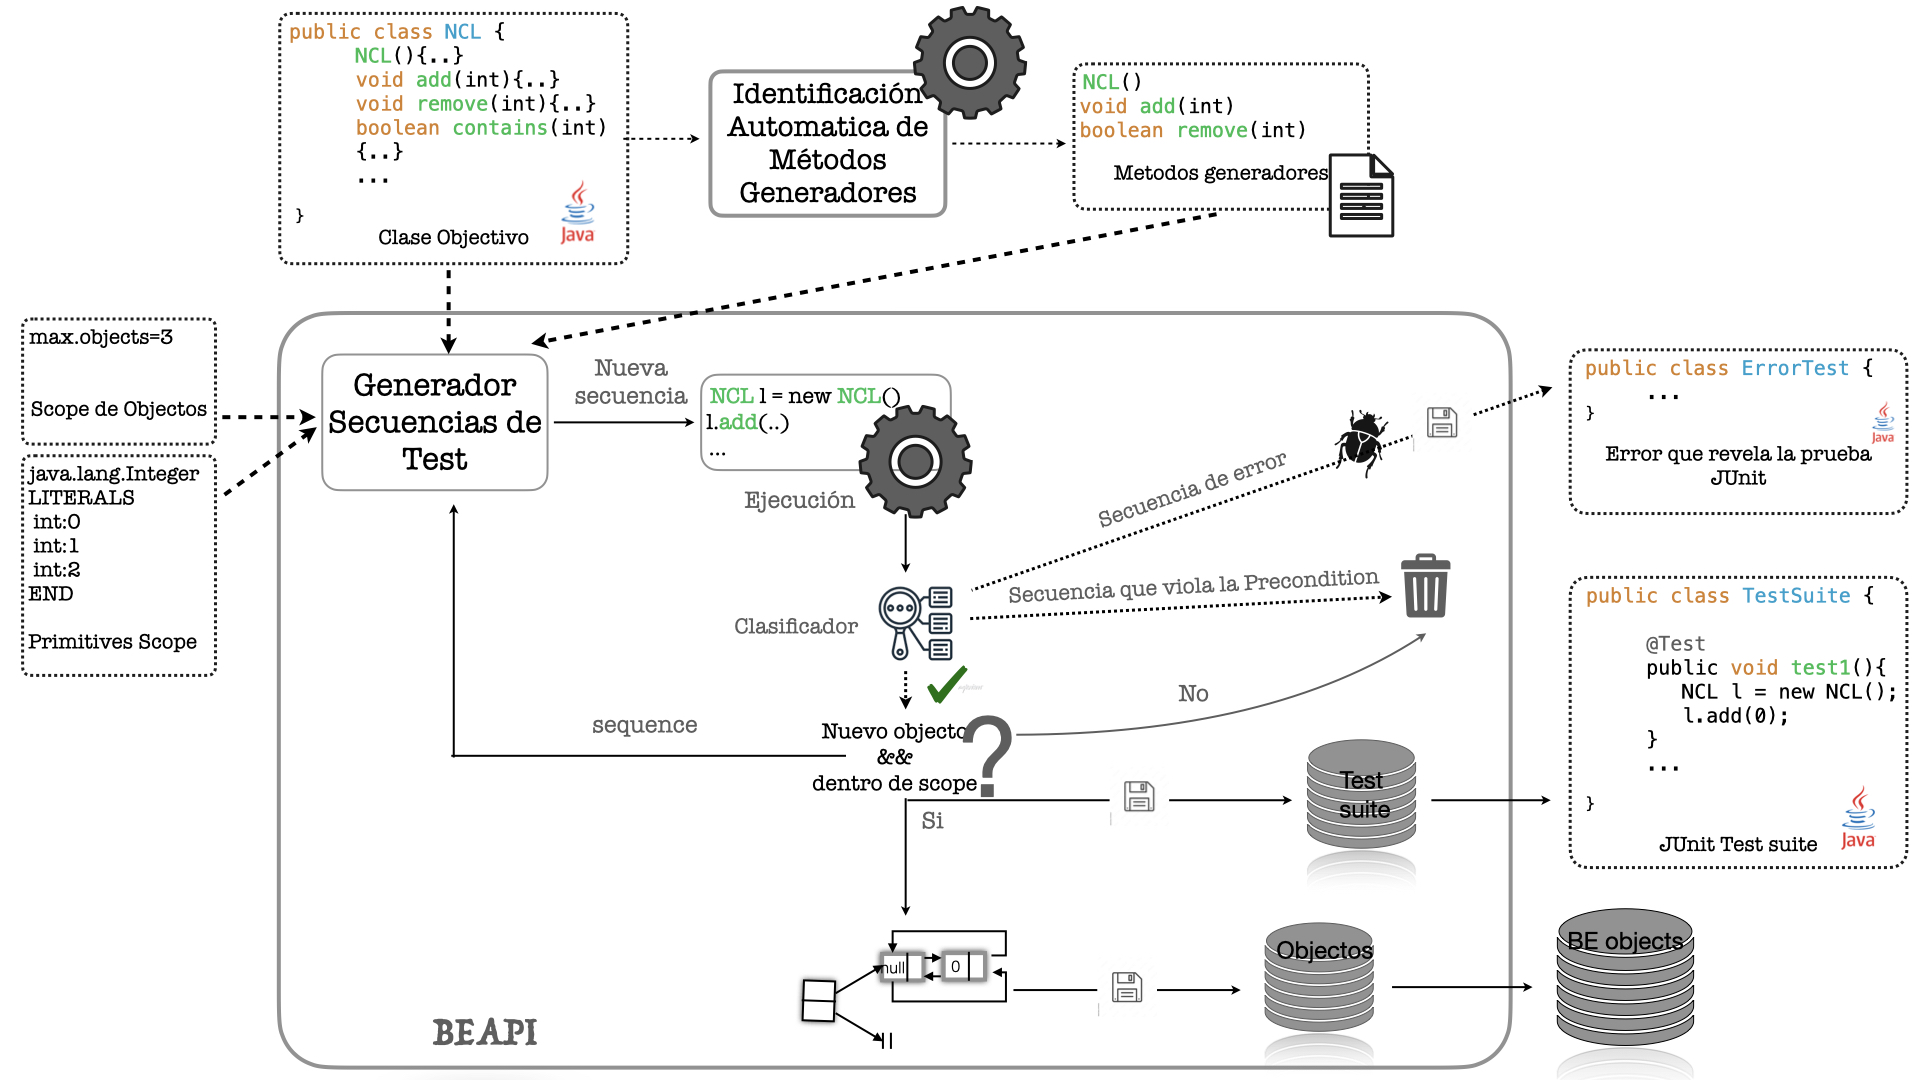
\includegraphics[width=1.0\textwidth]{images/beapi-arquitecture.jpeg}
  \caption{Visión general de la técnica \textsf{BEAPI}}
  \label{fig:beapi-overview}
\end{figure}

La Figura~\ref{fig:beapi-overview} muestra una visión general de la técnica 
\textsf{BEAPI} (\emph{Bounded Exhaustive generation from program APIs}), que implementa un enfoque 
de generación exhaustiva acotada de objetos mediante invocaciones a métodos de
la API de un módulo. 

% Entradas y salidas
Como entradas, \textsf{BEAPI} recibe:
\begin{itemize}
    \item la clase o clases objetivo para la generación de casos de prueba;
    \item archivos de configuración que definen los scopes de la generación
        exhaustiva acotada: tamaño máximo permitido para los objetos, y los valores primitivos 
        que se usarán para la generación;
    \item un archivo con los métodos de la clase objetivo que se emplearán 
        (por ejemplo, la API completa, o \emph{métodos generadores de objetos}).
\end{itemize}

Como salidas, \textsf{BEAPI} produce:
\begin{itemize}
    \item un conjunto exhaustivo acotado de objetos para los scopes dados;
    \item una suite de tests \texttt{JUnit}~\cite{junit} con las secuencias de test 
        que genera \textsf{BEAPI} para crear los objetos de salida del punto anterior;
    \item otra suite con tests que revelan errores (si los hubiera) en los métodos utilizados 
        para la generación.
\end{itemize}

\textsf{BEAPI} explota la idea de generación de tests dirigida por retroalimentación 
(\emph{feedback-directed test generation} \cite{Pacheco07,PaPacheco08}, ver Sección~\ref{sec:feedback-directed-test-gen}). 
Al igual que otros enfoques de generación de tests basados en la API, 
\textsf{BEAPI} construye secuencias de test \cite{Pacheco07,PaPacheco08}(secuencias de invocaciones a
métodos de la API), y las ejecuta para producir objetos.

%\textsf{BEAPI} aborda las dificultades de escribir especificaciones formales 
%para la generación exhaustiva acotada aprovechando la ejecución directa de las 
%rutinas de la API y aplicando técnicas de poda para mejorar la eficiencia y 
%permitir la escalabilidad a alcances mayores.

A grandes rasgos, el módulo \emph{generador de secuencias de test} (Figura~\ref{fig:beapi-overview}) 
comienza creando todas las secuencias de test posibles de longitud 1 (con una
única invocación a un método). Los valores primitivos definidos como parte del
scope son utilizados para instanciar los parámetros de los métodos en las
invocaciones.
El generador ejecuta cada secuencia, y aquellas que generan nuevos objetos (diferentes 
a los ya obtenidos, ver Sección \ref{sec:stateMatching}) son usadas por
el generador para producir nuevos tests, extendiendo dichas secuencias. A partir
de estas, se construyen secuencias de longitud 2, agregando una invocación
adicional a un método. 
Este proceso se repite iterativamente, generando secuencias de longitud 3, 4, y así sucesivamente.
El proceso continúa hasta que las secuencias de longitud $k$ no generan nuevos 
objetos (dentro de los scopes dados).
En ese punto, el generador de secuencias detiene su ejecución y BEAPI devuelve
la suite de tests generada junto con los objetos producidos.

% Clasificación de resultados
El módulo \emph{clasificador} observa el resultado de cada ejecución y clasifica 
la secuencia en una de cuatro categorías:
\begin{enumerate}
    \item La secuencia revela un error en algún método.
    \item La secuencia viola una precondición de un método.
    \item La secuencia genera un objeto que excede los límites permitidos por el alcance, o bien genera objetos que ya fueron producidos por secuencias anteriores.
    \item La secuencia genera al menos un nuevo objeto válido dentro del alcance permitido.
\end{enumerate}

Los casos (3) y (4) corresponden a ejecuciones exitosas, es decir, secuencias que finalizan sin lanzar excepciones. 
En estos casos, los objetos almacenados en las variables al finalizar la
ejecución de la secuencia de test son \emph{canonizados} \ref{sec:stateMatching}
y se verifica si ya han sido generados previamente, o si exceden los límites
permitidos por los scopes. 
Si esto último ocurre (caso 3), tanto la secuencia como los objetos que produce son descartados. 
En cambio, si la secuencia crea al menos un nuevo objeto válido (caso 4), 
entonces se retroalimenta al generador de secuencias para su potencial extensión
en el futuro, 
se almacena como caso de test en la suite retornada por BEAPI,
y los objetos generados se agregan al conjunto de objetos de salida.

Los casos (1) y (2) corresponden a ejecuciones que no finalizan correctamente y lanzan excepciones. 
Siguiendo la propuesta de Randoop~\cite{Pacheco07}, el tipo de excepción permite distinguir entre lo que BEAPI considera errores (o \emph{bugs}) 
y violaciones de precondiciones. 
Por defecto, BEAPI interpreta las excepciones \texttt{IllegalArgumentException} y \texttt{IllegalStateException} como violaciones de precondiciones, mientras que considera el resto de las
excepciones como errores en los métodos usados para la generación.
El comportamiento ante excepciones de BEAPI puede ser modificado mediante
parámetros de configuración de la herramienta. 
Las secuencias que violan precondiciones (caso 2) son descartadas, 
mientras que las secuencias que revelan errores (caso 1) 
son reportadas y retornadas al usuario. De forma similar a Randoop, 
es posible mejorar la capacidad de detección de errores proveyendo manualmente
especificaciones formales, como un método que implemente un predicado
\texttt{repOK} tal y como se describió en la sección anterior ~\cite{Pacheco07}.

BEAPI puede configurarse para habilitar o deshabilitar dos optimizaciones clave: 
la coincidencia de estados (ver Sección \ref{sec:stateMatching}) y el uso de métodos generadores de objetos
precomputados (ver Sección \ref{sec:buildersOptimization}) . 
Cuando estas optimizaciones están deshabilitadas, BEAPI puede resultar muy ineficiente 
y solo terminar en tiempos razonables para scopes pequeños (por ejemplo, scope 3). 
En cambio, con las optimizaciones habilitadas, el desempeño de BEAPI es comparable al de Korat (ver Capítulo \ref{cap:experimental}).

Si no hay fallas, BEAPI genera una suite de tests en formato \texttt{JUnit}. 
Cada test en la suite corresponde a una secuencia de métodos cuya ejecución
construye alguno(s) de los objetos en el conjunto exhaustivo acotado de objetos resultante.
%Otra ventaja de \textsf{BEAPI} es que, para cada objeto generado, proporciona una secuencia de test que se puede ejecutar para crear el objeto. 
Esto es una ventaja de BEAPI con respecto a los enfoques basados en
especificaciones (que generan un conjunto de objetos a partir de un \texttt{repOK}). 
Encontrar una secuencia de invocaciones a métodos de la API que construya una estructura específica es un problema difícil en sí mismo, 
y en particular es costoso computacionalmente \cite{Braione17}. Adicionalmente, requiere
de un esfuerzo importante si se lleva a cabo de manera manual. 
Por lo tanto, a menudo los objetos generados por enfoques basados en
especificaciones se "hardcodean" cuando se usan como entradas para test, por
ejemplo, mediante el uso de algún mecanismo como reflexión en Java. Esto hace
que los tests sean más difíciles de entender y mantener, ya que dependen de los
detalles de implementación de bajo nivel de las estructuras \cite{Braione17} (en
lugar de depender de la API de alto nivel).


% \pp{Esto no va acá. Va en una sección que se llama programación defensiva que
%     puede estar después de scope, y que se encarga de explicar esto, y cómo ejecutando un test
% se puede descartar una secuencia.}
% A diferencia de los enfoques de generación basados en caja negra, \textsf{BEAPI} no requiere una especificación formal de las propiedades de las estructuras. Al igual que otras técnicas de generación exhaustiva acotada (BEG), el usuario solo debe proporcionar los alcances para la generación, que se abordan en detalle en la sección correspondiente.  Esto permite generar estructuras válidas sin requerir una especificación detallada de las propiedades de las estructuras, reduciendo así la carga de trabajo para el programador.

% La principal ventaja de \textsf{BEAPI} es que requiere un esfuerzo menor de especificación para realizar la generación exhaustiva acotada. Si los métodos de la API utilizados en la generación son correctos, todas las estructuras generadas serán válidas para su construcción. El programador solo necesita asegurarse de que los métodos de la API lancen excepciones cuando se violen las reglas de uso, siguiendo un estilo de programación defensivo \cite{Liskov00}. En la mayoría de los casos, esto implica verificar condiciones muy simples en las entradas. Por ejemplo, el método para eliminar (\emph{remove(int)}) un elemento de una \texttt{NCL} en un índice pasado como parámetro lanza una \texttt{IllegalArgumentException} cuando se llama con un índice menor a 0 o mayor al \emph{size} de la lista. El \emph{listing} de la figura \ref{fig:algoProgDefensiva}  se puede observar que la implementación del método se encarga de cumplir con la especificación indicada \texttt{NCL}.
% Para hacer esto

\section{Scope}
\label{sec:scope}

En el contexto de la generación exhaustiva acotada, el término \emph{scope} se
refiere a los límites en los dominios de datos que se imponen para la generación de
estructuras. 
Así, el scope es esencial para controlar el tamaño y la complejidad del espacio de búsqueda de estructuras. 
Sin un límite para los tamaños las estructuras generadas,
 el espacio de búsqueda podría ser extremadamente grande o infinito, lo que haría
 que la generación exhaustiva sea impracticable en la mayoría de los casos. 

Para la definición de los scopes BEAPI requiere de un archivo de configuración
simple en formato \texttt{java.properties}. En la Figura \ref{fig:NCL-fin-BEAPI}
se muestra un ejemplo de este archivo. 
La variable \emph{max.objects} permite definir el número
máximo de objetos que se pueden crear para cada clase. En el ejemplo de la
Figura, \emph{max.objects=3} indica que BEAPI sólo admitirá secuencias de test que
generen listas con hasta 3 objetos de tipo NCL, y 3 objetos de tipo Node. Las
secuencias de test que crean estructuras que 
exceden estos límites (para cualquier clase) se descartan, al igual que los
objetos creados por las mismas por exceder los scopes. Como ejemplo, la Figura
\ref{sec:scope} muestra una secuencia de test generada usando el método constructor
de la clase NCL, y el método \emph{add}. Recordar que estamos considerando un scope de 3. 
Esto quiere decir que cuando se genera alguna estructura con más de 3 nodos, como es en 
el caso de la última secuencia de test de la Figura, esta es descartada por exceder el 
límite de nodos en la estructura (notar que el nodo ficticio de la estructura cuenta como un
nodo).


%\begin{figure}[H]
%    \centering
%    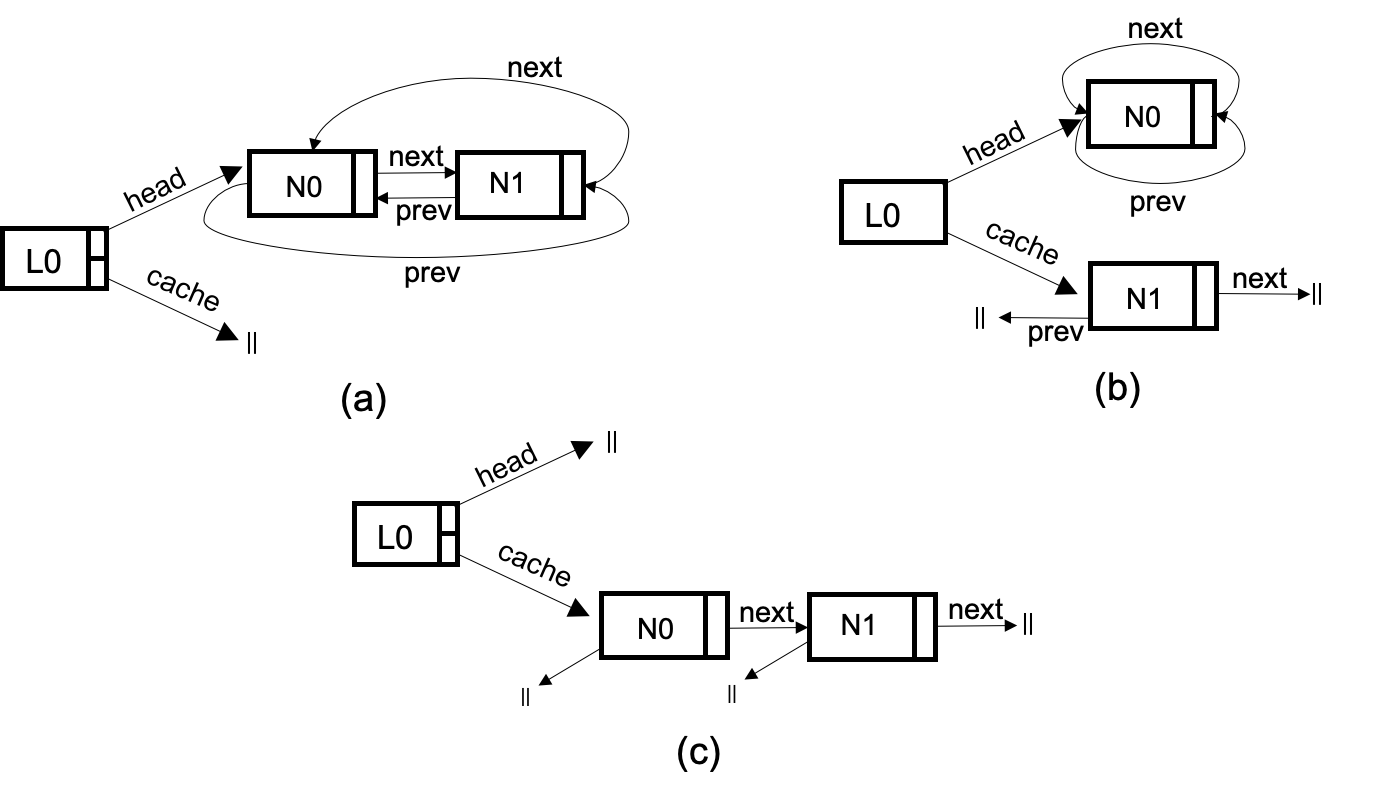
\includegraphics[width=0.85\textwidth]{images/NCL-instances.png}
%    \caption{Tres instancias de NodeCachingLinkedList con exactamente dos nodos}
%    \label{fig:ncl-instances}
%\end{figure}
%\pp{Esta figura es igual a la Figura 2? Digo porque hay otra con instancias
%antes? Si la vamos a repetir en este capítulo capaz que convenga ponerla antes y
%eliminar la otra?}

\begin{figure}[H]
\begin{lstlisting}[keywordstyle=\scriptsize\ttfamily]
max.objects=3
int.range=0:2
strings=str1,str2,str3
omit.fields=DEFAULT_MAXIMUM_CACHE_SIZE
\end{lstlisting}
\caption{Definición del scope de BEAPI para NCL (nodos max. 3)}
\label{fig:NCL-fin-BEAPI}
\end{figure}


Nuestra técnica, basada en generación de tests guíada por feedback, necesita un
conjunto de valores primitivos (enteros, strings, etc.) provisto por el usuario
que son utilizados para invocar a los métodos de la API con parámetros de
tipos primitivos. En las líneas 2 y 3 de la Figura \ref{fig:NCL-fin-BEAPI} se
definen los valores de tipo enteros y String, respectivamente, que serán utilizados por los métodos 
cuando necesiten valores de estos tipos. En la Figura se definen enteros en un
rango que va del 0 al 2, y las cadenas de caracteres ``str1'', ``str2'' y 
``str3''. Ademas, se pueden proveer valores para todos los tipos incluyendo floats, doubles, etc. 
Esto serán los dominios de datos para los tipos primitivos que tomen como
parámetros los métodos que serán utilizados durante la generación.
Por ejemplo, el método \emph{add(int)} de NCL, que agrega un elemento al final de la lista
principal, necesita del entero que será almacenado en el campo \emph{value} del nuevo nodo. 
Dado el archivo de configuración de la Figura \ref{fig:NCL-fin-BEAPI}, cada vez
que deba invocar al método \emph{add}, BEAPI lo llamará instanciando su parámetro con los valores 0,
1 y 2.

\begin{figure}[H]
    \centering
    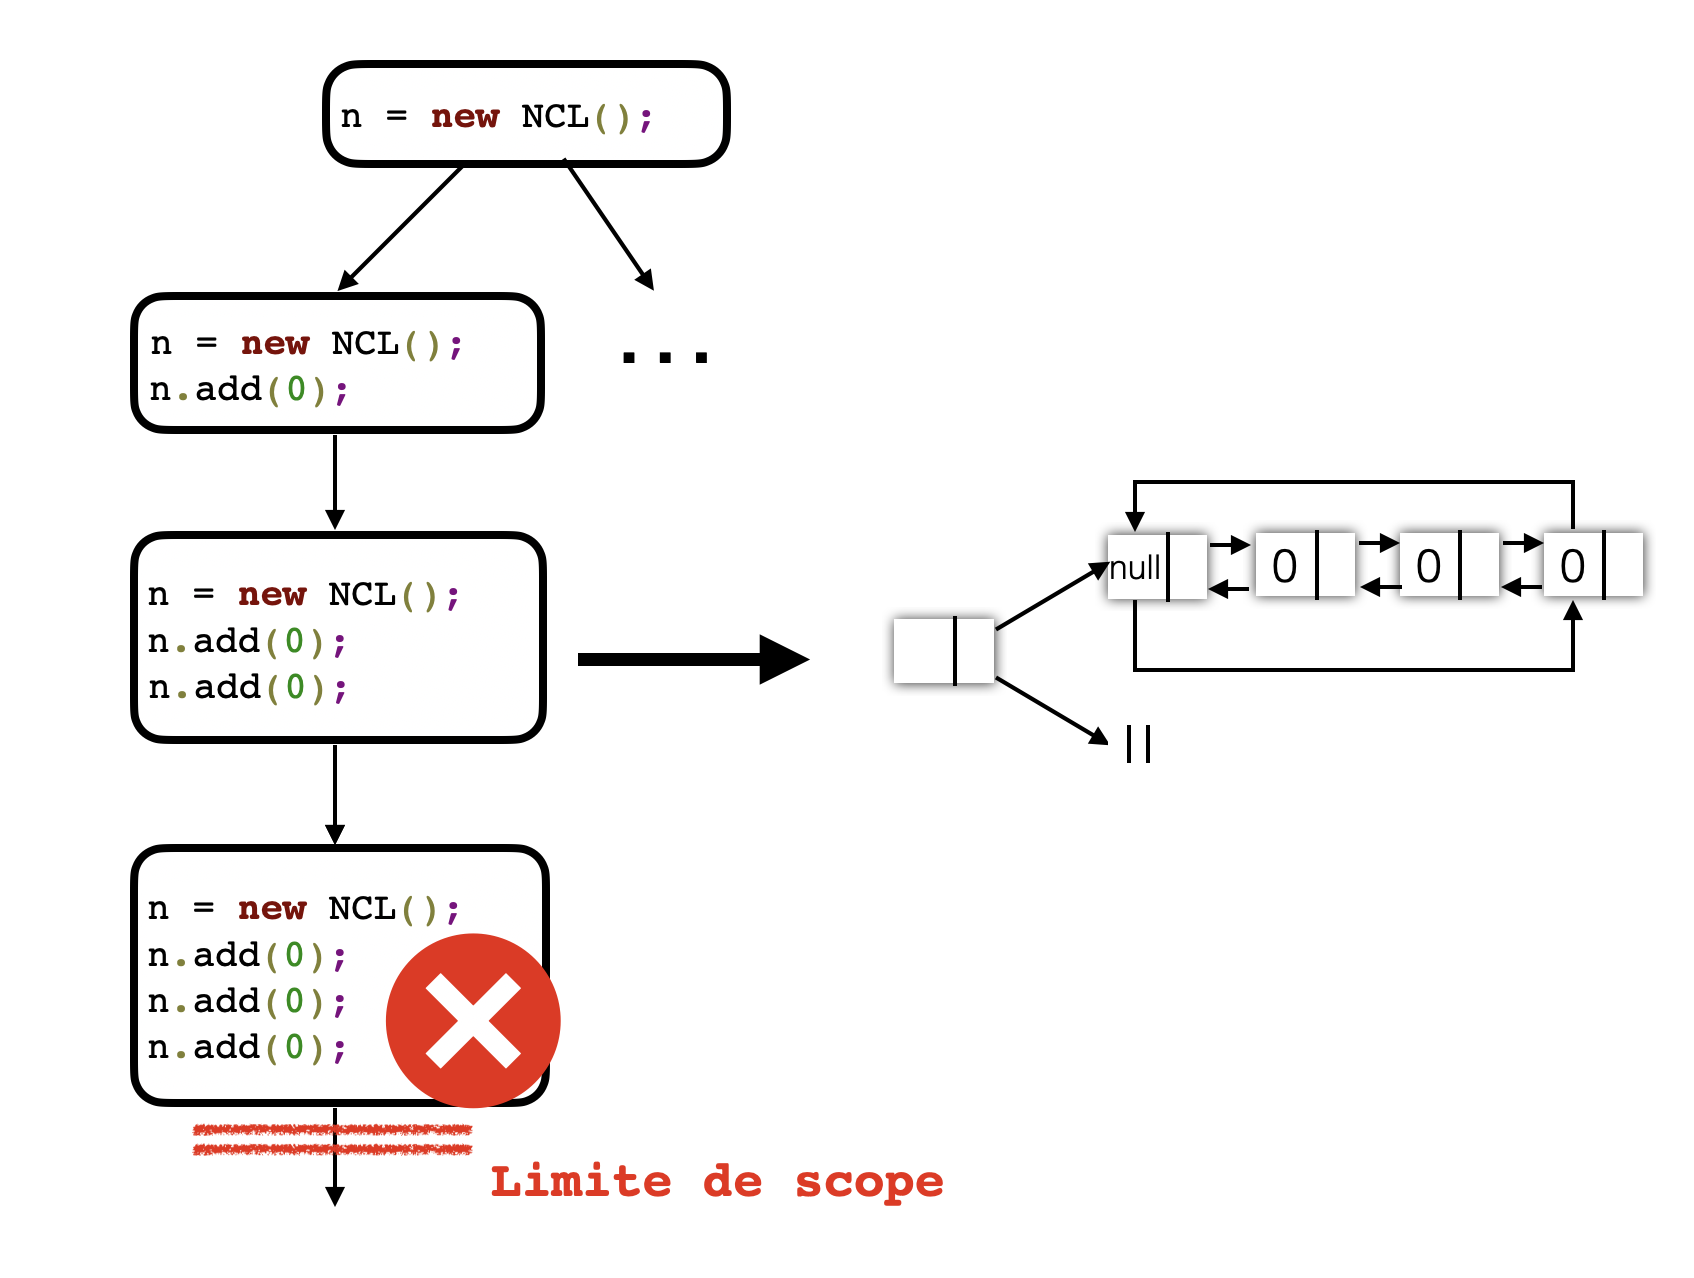
\includegraphics[width=0.85\textwidth]{images/scope.jpg}
    \caption{Secuencia de test descartada por exceder la máxima cantidad de
    nodos (scope 3) para NCL}
    \label{fig:scope}
\end{figure}

% Siguiendo el análisis del archivo de configuración de la figura \ref{fig:NCL-fin-BEAPI},
% y el número de valores primitivos disponibles, en nuestro ejemplo de la figura, 


Podemos indicarle a \emph{BEAPI} que ignore algunos campos en el proceso de
linealización de objetos (ver más adelante en la sección
\ref{sec:stateMatching}), que se lleva a cabo luego de la ejecución de las
secuencias de test. Esto permite al usuario controlar qué partes de la
estructura del objeto son relevantes para la coincidencia de estados. Por
ejemplo, la línea 4 hace que \emph{BEAPI} omita el tamaño máximo predeterminado
de la caché en la coincidencia de estados, que en \emph{NCL} es una
constante inicializada en 20 en el constructor de la clase. En general, \texttt{omit.fields}
toma una expresión regular en Java, y \emph{BEAPI} omite los campos de las clases
cuyo nombre \emph{matchean} con la expresión regular. Es importante que
aquí se omitan campos que puede afectar negativamente la coincidencia de
estados.
Por ejemplo, \emph{modCount} es un campo de tipo entero que se incrementa 
cada vez que se realiza una modificación en las estructura de datos
provistas por \texttt{java.util}. Las modificaciones pueden incluir 
inserciones, eliminaciones, actualizaciones u otras operaciones que afecten la colección. 
El propósito principal de llevar un contador de modificaciones es facilitar la detección de modificaciones concurrentes o cambios inesperados en la colección por parte de múltiples hilos de ejecución. 
Sin embargo, para los propósitos de la generación exhaustiva acotada considerar \emph{modCount} como un
campo de la estructura puede hacer que muchas listas que en contenido son iguales sean diferentes
por tener distintos valores para este campo (por ejemplo, porque se les
aplicaron una cantidad distinta de operaciones). Esto haría crecer
innecesariamente la cantidad de estructuras generadas por \emph{BEAPI}, sin
brindar ningún beneficio desde el punto de vista del testing estructural.
Por lo tanto, el usuario puede omitir \emph{modCount} definiendo una expresión 
regular para \texttt{omit.fields}
(\texttt{DEFAULT\_MAXIMUM\_CACHE\_SIZE|modCount}).



%Cómo último, nuestro archivo de configuración, permite que el usuario especifique que valores desea que no sean tenidos en cuenta a la hora de comparar estructuras. 
%Esto toma especial importancia el contexto de estructuras de datos, especialmente en colecciones y contenedores en Java. En estos casos suelen aparecer campos en la clase que representa un contador de modificaciones o cambios realizados en la estructura de datos. Comúnmente son llamados \emph{modCount}. 
%Este es un campo que se utiliza para realizar un seguimiento de las modificaciones que se han realizado en la colección desde su creación o desde la última vez que se realizó un seguimiento. 
%
%En la línea 4 del archivo de configuración \ref{fig:NCL-fin-BEAPI}, se puede observar como se especifica aquellos campos que deseamos omitir a la hora de tener una representación canónica de la estructura. Canonicalizar un objeto se refiere a la acción de garantizar que un objeto se encuentre en su forma más básica y representativa, lo que facilita las comparaciones y operaciones con otros objetos similares.
%Para lograr todo lo explicado en esta sección, nosotros canonizamos los objetos generados por la ejecución de cada secuencia de métodos y analizamos y trabajamos con su representación canónica.
%



% \pp{Esta canonización no coincide con la que se explica en state matching, que
%     implica recorrer un grafo y generar una secuencia. Yo no sé si pondría este
% ejemplo. De cualquier modo, no va acá en la sección de scope, de última va para
% state matching. Yo cerraría la sección acá.}
% Imaginemos un conjunto de números representado en diferentes órdenes:
% \begin{itemize}
%     \item Conjunto 1: \{3, 1, 2\}
%     \item Conjunto 2: \{1, 2, 3\}
%     \item Conjunto 3: \{2, 3, 1\}
% \end{itemize}

% Aunque los elementos de cada conjunto son los mismos, el orden de los números varía. Si quisiéramos comparar estos conjuntos para determinar si son equivalentes, el proceso de canonización podría consistir en ordenar los números en cada conjunto de manera ascendente:

% \begin{itemize}
%     \item Conjunto 1 canonizado: {1, 2, 3}
%     \item Conjunto 2 canonizado: {1, 2, 3}
%     \item Conjunto 3 canonizado: {1, 2, 3}
% \end{itemize}

% Tras la canonización, todas las versiones del conjunto resultan idénticas, lo que nos permite determinar fácilmente que los tres conjuntos son equivalentes, independientemente del orden en el que aparecían originalmente los números.

% En el contexto de estructuras de datos, este proceso podría implicar reorganizar los nodos, normalizar los valores de ciertos campos, o eliminar detalles que no son relevantes para la comparación, como el \emph{modCount} mencionado anteriormente. Al canonizar, se asegura que dos estructuras de datos se comparen en términos de su contenido esencial, ignorando diferencias superficiales o de implementación.

% (Normalmente, las técnicas basada en generación por retroalimentación guardaría los valores primitivos que son devueltos por la ejecución de las pruebas y reutilizaría estos valores en pruebas futuras). 
% También nuestra técnica descartar secuencias de métodos que crean objetos con más de $k$ objetos (de cualquier tipo), para evitar que se construyan objetos más grandes de lo necesario. 


% \cacho{VER BIEN ESTO DE NO EXTENDERSE, porq para crear estrucutras de 3 nodos a veces necesito crear previamente una de 4 nodos}
% Esto asegura que se generen solo \texttt{NCL} con no más de k nodos. 
% Por ejemplo, la figura \ref{fig:scope}, se puede observar que cuando genera una estructura con mas nodos que el especificado en el archivo de configuración, 
% este no sigue extiendo el árbol de búsqueda. En la figura el scope especificado es 3 (vale aclarar, que el nodo ficticio cuanta como nodo de la estructura.)


\section{Programación Defensiva}
\label{sec:defensiveProgramming}

Una de las principales ventajas del enfoque \textsf{BEAPI} frente a otras
técnicas de generación exhaustiva acotada existentes 
es que no requiere de especificaciones formales adicionales (como 
un \texttt{repOK}).
En lugar de depender de especificaciones complejas como el \texttt{repOK} de la
Figura \ref{fig:NCL-repOK} (como ocurre con \textsf{Korat}), \textsf{BEAPI} se
apoya en la asunción de que los métodos de la API que se usan para la generación
(por ejemplo, los generadores de objetos) sólo construyen objetos correctos.
Típicamente, esto es posible gracias a la adopción del estilo llamado
\emph{programación defensiva}~\cite{Liskov00} en la definición de los métodos. 
La programación defensiva es una técnica que promueve la verificación de
precondiciones en los métodos públicos de la API, de modo que los errores 
relacionados con el uso incorrecto de la API puedan ser detectados y reportados
mediante las excepciones apropiadas.

En el contexto de \textsf{BEAPI}, esta práctica permite descartar automáticamente secuencias de métodos que violan las restricciones de uso 
de la API, ya que los tests generados que invocan métodos con parámetros inválidos o en estados inconsistentes provocan una excepción 
durante la ejecución. Dado que \textsf{BEAPI} ejecuta cada secuencia como parte del proceso de exploración, este mecanismo actúa 
como un filtro dinámico: las secuencias de test que lanzan excepciones correspondientes
a violaciones de precondiciones no se consideran como candidatas para generar nuevas estructuras.

\begin{figure}[!htb]
\begin{lstlisting}
public Object removeIndex(int index) {
  // Verificacion de precondicion
  if(index < 0 || index >= size)
      throw new IllegalArgumentException();  
  // Codigo omitido
}
\end{lstlisting}
\caption{Programación defensiva en un metodo en \texttt{NodeCachingLinkedList}.}
\label{fig:algoProgDefensiva}
\end{figure}

El código mostrado en la Figura~\ref{fig:algoProgDefensiva} ejemplifica la
técnica de programación defensiva. 
El método \texttt{removeIndex} de la clase \texttt{NodeCachingLinkedList} verifica que el índice especificado se encuentre dentro de los límites de la lista. 
Si la condición no se cumple, se lanza una excepción que permite a
\textsf{BEAPI} descartar automáticamente la secuencia correspondiente (sin
necesidad de especificar esta restricción en un invariante externo).

Este enfoque reduce significativamente la carga de trabajo del usuario, ya que no es necesario escribir un \texttt{repOK} manual ni mantenerlo 
en sincronía con la implementación cuando se realizan cambios sobre la misma. En
cambio, basta con asegurar que los métodos de la API respeten buenas prácticas
de verificación de precondiciones sobre las entradas. 
De este modo, \textsf{BEAPI} puede aprovechar la ejecución dinámica de los tests para delimitar correctamente el espacio de estructuras válidas.


\section{Coincidencia de estados}
\label{sec:stateMatching}
Esta optimización nace de la observación de que durante la generación exhaustiva
acotada con \textsf{BEAPI} pueden surgir múltiples de secuencias de test que
construyen el mismo objeto. 
Estas secuencias redundantes aumentan el espacio de exploración
de \textsf{BEAPI}, malgastando tiempo de CPU e incrementando significativamente el 
tiempo de ejecución de la técnica. 
Para mitigar este problema, \textsf{BEAPI} implementa una estrategia de
coincidencia de estados (\emph{state matching} en inglés) que permite
identificar y descartar secuencias de test que conducen a objetos generados
previamente.

Por ejemplo, crear una lista vacía, agregar un elemento, eliminarlo y luego volver a agregarlo, resulta en el mismo estado que simplemente agregar ese elemento a una lista vacía. 
De manera similar, intentar eliminar un elemento de una lista vacía no altera su estado, produciendo el mismo resultado que una lista recién creada. 
En estructuras como pilas, realizar una operación de \texttt{push}, seguida de un \texttt{pop} y un nuevo \texttt{push} del mismo valor, 
produce una configuración indistinguible de aquella que resulta de realizar únicamente el último \texttt{push}. 

Este tipo de situaciones son capturadas por la estrategia de coincidencia de
estados, que consiste en almacenar las estructuras generadas durante la
exploración, y descartar cualquier nueva secuencia de test que produzca una
estructura ya generada. 
\textsf{BEAPI} asume que las ejecuciones de los métodos de la API son
deterministas, es decir, que cualquier ejecución de un método con las mismas entradas produce 
siempre el mismo resultado. 
Por lo tanto, si una secuencia de test conduce a la creación de estructuras
que ya han sido generadas por una secuencia anterior, no es necesario seguir
extendiendo la nueva secuencia con sucesivas invocaciones a otros métodos, ya 
que esto no producirá nuevos objetos distintos.

En la Figura~\ref{fig:stateMatching}, se puede observar de manera más clara este
problema de generación de estructuras redundantes.
Cada nodo del árbol representa una secuencia test generada por \texttt{BEAPI}
para \texttt{NodeCachingLinkedList}. 
Las flechas indican la extensión de una secuencia de test agregando una nueva
operación al final de la secuencia previa.
Las marcas de \emph{visited state} indican que el objeto ya fue generado por
secuencias previas.
Esta Figura ilustra claramente que típicamente hay múltiples formas de obtener
la misma estructura usando la API.

\begin{figure}[H]
  \centering
  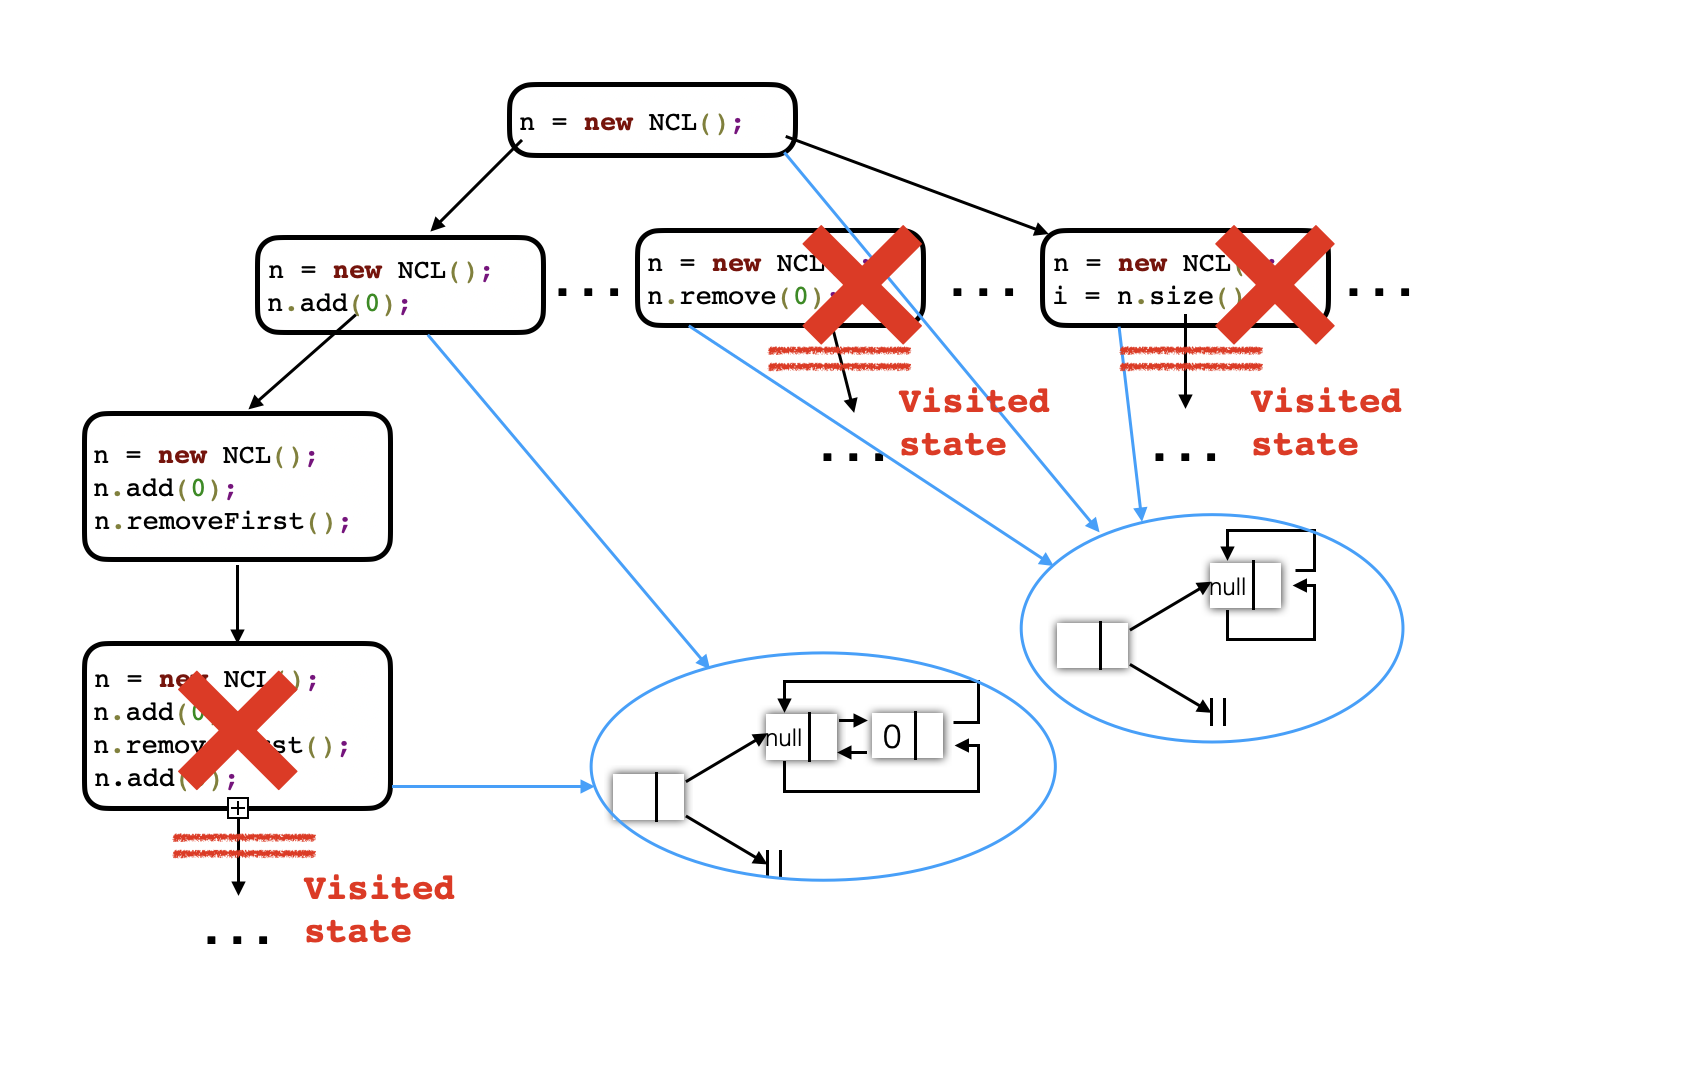
\includegraphics[width=1\textwidth]{images/stateMatching1.jpg}
  \caption{State matching en \emph{NodeCachingLinkedList}}
  \label{fig:stateMatching}
\end{figure}

La coincidencia de estados es, por lo tanto, una optimización crítica para que
la generación exhaustiva acotada pueda funcionar para problemas con APIs ricas
en cantidad de métodos, ya que las combinaciones posibles de métodos para
construir objetos crecen exponencialmente con la cantidad de métodos
disponibles.
Implementamos esta técnica en \textsf{BEAPI} mediante la transformación de las
estructuras generadas a una representación canónica, que permite almacenar las  
estructuras y compararlas por igualdad eficientemente \cite{Iosif02,Xie04}. El procedimiento se
describe a continuación.

%Concretamente, \textsf{BEAPI} almacena todas las estructuras generadas hasta el momento en su forma canónica. 
%Luego de ejecutar la última rutina \texttt{r(p$_1$, ..., p$_k$)} de una nueva secuencia de prueba \texttt{T}, 
%el sistema verifica si alguno de los parámetros involucrados en \texttt{r} posee una estructura que no haya sido observada previamente (es decir, que no esté almacenada). 
%Si ninguna estructura nueva es detectada, la secuencia \texttt{T} se considera redundante y es descartada. 
%De lo contrario, \texttt{T} se almacena como secuencia representativa, junto con las nuevas estructuras producidas.

Formalmente, representamos las estructuras almacenadas en el heap como grafos
etiquetados con un nodo raíz, denominados heaps con raíz. 
Después de la ejecución de un método, un parámetro $p$ de tipo no primitivo
(incluyendo al receptor \texttt{this}) contiene una referencia al objeto raíz $r$ de un
heap con raíz, es decir, $p=r$.

\begin{definition}
Sea $O$ un conjunto de objetos y $P$ un conjunto de valores primitivos (incluido $null$). Sea $F$ el conjunto de campos de todos los objetos en $O$.
\begin{itemize}
\item Un \emph{heap} es un grafo etiquetado $H = \langle O, E\rangle$ con $E =
    \{(o, f, v) | o \in O, f \in F, v \in O \cup P\}$.
\item Un \emph{heap con raíz} es un par $RH = \langle r, H \rangle$ donde $r \in
    O$, $H = \langle O, E\rangle$ es un heap, y para cada $v' \in O \cup P$,
    $v'$ es alcanzable desde $r$ a través de los atributos $f \in F$.
\end{itemize}
\end{definition}

El caso especial $p = null$ se representa con un heap con raíz que tiene un nodo
ficticio y un campo ficticio que apunta a $null$. En lenguajes como Java, cada
objeto se identifica por la dirección de memoria donde se encuentra. Cambiar las
direcciones de memoria donde se almacenan los objetos no tiene efecto desde el
punto de vista del programa, ya que el programador no tiene control sobre la
representación de bajo nivel de la memoria (a diferencia de otros lenguajes como
C). Los heaps obtenidos mediante permutaciones de las direcciones de memoria de
sus objetos componentes se llaman \emph{heaps
isomorfos}\cite{Iosif02,Boyapati02}. Evitamos la generación de \emph{heaps
isomorfos} empleando una representación canónica para los heaps. Los heaps con
raíz se pueden canonizar eficientemente mediante un enfoque llamado
\emph{linearización} \cite{Iosif02,Xie04}, que convierte un heap con raíz en
una secuencia de valores primitivos que lo representa de forma canónica.

\bigbreak

% \begin{figure}[!th]
% \begin{lstlisting}
% int[] linearizar(O raiz, Heap<O, E> heap, int alcance, Regex omitirCampos) {
%     Map ids = new Map(); // mapea nodos a sus identificadores unicos
%     return lin(raiz, heap, alcance, ids, omitirCampos);
% }
% int[] lin(O raiz, Heap<O, E> heap, int alcance, Map ids, Regex omitirCampos) {
%     if (ids.containsKey(raiz))
%         return secuenciaUnica(ids.get(raiz));
%     if (ids.size() == alcance)
%         throw new excepcionAlcanceSuperado();
%     int id = ids.size() + 1;
%     ids.put(raiz, id);
%     int[] seq = secuenciaUnica(id);
%     Edge[] campos =
%     ordenarPorCampo({ <raiz, f, o> en E }, omitirCampos);
%     foreach (<raiz, f, o> en campos) {
%         if (esPrimitivo(o))
%             seq.add(representacionUnica(o));
%         else
%             seq.append(lin(o, heap, alcance, ids, omitirCampos));
%     }
%     return seq;
% }
% \end{lstlisting}
% \caption{Algoritmo de linearización}
% \label{alg:linearization}
% \end{figure}



\begin{figure}[!th]
\begin{lstlisting}
int[] linearize(O root, Heap<O, E> heap, int scope, Regex omitFields) {
    Map ids = new Map(); // maps nodes into their unique ids 
    return lin(root, heap, scope, ids, omitFields); 
}
int[] lin(O root, Heap<O, E> heap, int scope, Map ids, Regex omitFields) { 
  if (ids.containsKey(root))
    return singletonSequence(ids.get(root)); 
  if (ids.size() == scope) 
    throw new ScopeExceededException();
  int id = ids.size() + 1;
  ids.put(root, id);
  int[] seq = singletonSequence(id);
  Edge[] fields = sortByField({ <root, f, o> in E }, omitFields); 
  foreach (<root, f, o> in fields) {
    if (isPrimitive(o)) 
      seq.add(uniqueRepresentation(o));
    else
      seq.append(lin(o, heap, scope, ids, omitFields));
  }
  return seq; 
}
\end{lstlisting}
\caption{Algoritmo de linealización}
\label{alg:linearization}
\end{figure}
% java.util.LinkedList.MAX_ARRAY_SIZE&java.util.LinkedList:0&2147483639
% java.util.LinkedList.first&java.util.LinkedList:0&java.util.LinkedList$Node:0
% java.util.LinkedList.last&java.util.LinkedList:0&java.util.LinkedList$Node:1
% java.util.LinkedList.modCount&java.util.LinkedList:0&2
% java.util.LinkedList.serialVersionUID&java.util.LinkedList:0&876323262645176354
% java.util.LinkedList.size&java.util.LinkedList:0&2
% traversal.DummyHeapRoot.theroot&traversal.DummyHeapRoot:0&java.util.LinkedList:0


La Figura\ref{alg:linearization} muestra el algoritmo de linealización utilizado
por \textsf{BEAPI}, una versión modificada del algoritmo original para reportar
cuando los objetos exceden el \emph{scope}, e ignorar ciertos campos de los objetos (para la versión original, véase 
\cite{Xie04}). El procedimiento \texttt{linearize} inicia un recorrido en
profundidad del heap a partir de la raíz, invocando 
\texttt{lin} en la línea 3. Para canonizar el heap, \texttt{lin} asigna
identificadores únicos a cada objeto nuevo que visita. El mapa 
\texttt{ids} almacena la correspondencia entre objetos visitados y sus
identificadores asignados.

Cuando un objeto es visitado por primera vez, se le asigna un nuevo identificador (líneas 10--11), y se crea una secuencia \emph{singleton}
que representa dicho objeto (línea 12). A continuación, se recorren los
atributos del objeto, ordenados en un orden predefinido (en BEAPI los campos se
ordenan alfabéticamente por nombre), y se construye la linealización del valor
de cada atributo (líneas 13--19). Si un atributo contiene un valor primitivo, se lo representa mediante una secuencia singleton con dicho 
valor (líneas 15--16). Si un atributo hace referencia a otro objeto, se realiza una llamada recursiva a \texttt{lin} para convertir dicho objeto 
en una secuencia, la cual se añade al final de la secuencia resultado (línea
18). Al finalizar el ciclo, \texttt{seq} contiene la representación canónica del 
heap con raíz \texttt{root}, que se devuelve como resultado (línea 20).

Cuando un objeto ya visitado es alcanzado por una llamada recursiva, el mismo ya debe tener un identificador asignado en \texttt{ids} 
(línea 6), y \texttt{lin} retorna la secuencia singleton correspondiente (línea 7). Si durante el proceso se detecta que la cantidad de 
objetos alcanzables desde la raíz excede el \emph{scope} permitido, se lanza una excepción \texttt{ScopeExceededException} (líneas 9--10). Esta 
excepción será utilizada por \textsf{BEAPI} para descartar aquellas secuencias
de test que generan objetos más grandes que lo permitido por los \emph{scope}.

El procedimiento \texttt{linearize} también recibe como parámetro una expresión regular \texttt{omitFields}, que define los nombres 
de los atributos que deben ser ignorados durante la linealización. Para omitir estos 
atributos, la función \texttt{sortByField} (línea 13) ha sido implementada de forma tal que no devuelve las aristas correspondientes a 
los atributos cuyo nombre coincide con \texttt{omitFields}. Esto evita que los
valores de dichos atributos se incluyan en la secuencia resultante.

Finalmente, la linealización permite comparar estructuras de manera eficiente:
dos objetos (es decir, dos heaps con raíz) son iguales 
si y solo si las secuencias generadas por \texttt{linearize} para ambos son
iguales (comparando elemento a elemento).

Cabe destacar que por simplicidad el algoritmo presentado en la Figura\ref{alg:linearization} 
asume que los objetos almacenan enteros y retorna secuencias de enteros como representaciones
canónicas. El algoritmo implementado en BEAPI es más general, soporta objetos de
cualquier tipo y los representa como secuencias de Strings.

\section{Uso de m\'etodos generadores de objetos}
\label{sec:buildersOptimization}
En esta sección, se describe una optimización clave para BEAPI que hemos desarrollado y que es
una contribución principal de esta tesis (ver Capítulo \ref{cap:builders}).
Se observa que los métodos generadores de objetos nos permiten crear cualquier
instancia posible que se puede construir con la API, incluso de manera
exhaustiva acotada, es decir, generando todos los objetos posibles para un scope dado.
Dado que la cantidad de combinaciones de invocaciones a métodos crece de manera
exponencial con el número de métodos, es crucial reducir la cantidad de métodos
que \textsf{BEAPI} utiliza para producir secuencias de test. 

Para abordar este problema, se propone utilizar algún enfoque de identificación
automática de métodos generadores de objetos previo a la ejecución de BEAPI. 
Este enfoque nos permitirá encontrar un subconjunto pequeño de métodos de la API que son
suficientes para la generación exhaustiva acotada.
Luego, los generadores de objetos son pasados como parámetro a BEAPI como los
únicos métodos que debe utilizar (ver Figura \ref{fig:beapi-overview}). 
Esto reduce significativamente la cantidad de
secuencias que BEAPI necesita explorar, mejorando significativamente la
eficiencia de la técnica.

En el contexto de \textsf{BEAPI}, utilizamos el algoritmo de búsqueda basado en
\emph{escalada de colinas} (ver Sección \ref{sec:approachHC}), que logra un mejor rendimiento en tiempo de
ejecución. 
Aunque la \emph{escalada de colinas} puede ser menos preciso en algunos casos,
ya que puede incluir algunos métodos que no son necesarios entre los generadores
de objetos retornados, en nuestros experimentos el algoritmo funcionó muy bien y
computó consistentemente conjuntos suficientes de métodos generadores (ver
Sección \ref{sec:experimentalIdentificacion}. 
% Nuestro objetivo aquí es evaluar el impacto de utilizar builders para la generación exhaustiva acotada (BEG) a partir de una API.
Para la identificación de métodos generadores, utilizamos como función objetivo
a BEAPI como generador exhaustivo acotado. Esta función objetivo se explicó en
detalle en la Sección \ref{sec:fitnessGE}.

La idea clave que hace factible la identificación eficiente de métodos generadores
previamente a la generación exhaustiva acotada es que a menudo utilizar un
\emph{scope} relativamente pequeño es suficiente para identificar métodos
generadores de objetos que resultan ser los generadores de objetos para el caso
general (es decir, sin restricciones de scope).
%En otras palabras, una vez que el scope para el cómputo de los métodos generadores es lo suficientemente grande, aumentar el alcance producirá como resultado el mismo conjunto de constructores. 
Este resultado se asemeja a la ``hipótesis de la cota pequeña'', que predica que
para encontrar la mayor parte de las fallas es suficiente ejercitar el software
con estructuras de tamaño relativamente pequeño \cite{Andoni02}. También es
similar a la técnica llamada \emph{transcoping}, propuesta en \cite{Rosner13}.
En todos nuestros casos de estudio, un \emph{scope} de 5 fue suficiente para
computar los métodos generadores de objetos con precisión (ver Sección
\ref{sec:experimentalIdentificacion}.
Después de identificar eficientemente los métodos generadores usando un scope
pequeño, podemos ejecutar \textsf{BEAPI} con métodos generadores identificados
como parámetro utilizando scopes más grandes. Esto permite que \textsf{BEAPI}
produzca objetos más grandes, y con ellos es posible ejercitar más exhuastivamente 
el software bajo test.

\section{Algoritmo de BEAPI}
\label{sec:beapiTechnique}

\begin{figure}[ht]
\begin{lstlisting}
BEAPI(List methods, int scope, Map<Type, List<Seq>> primitives, Regex omitFields) {
  Map<Type, List<Seq>> currSeqs = new Map();
  currSeqs.addAll({ T->L | T->L in primitives });
  Set canonicalStrs = new Set();
  for (int it=0; true; it++) {
    Map<Type, List<Seq>> newSeqs = new Map();
    boolean newStrs = false;
    for (m(T$_1$,$\ldots$,T$_n$):T$_r$: methods) {
      Map<Type, List<Seq>> seqsT$_1$ = currSeqs.getSequencesForType(T$_1$);
      $\ldots$ 
      Map<Type, List<Seq>> seqsT$_n$ = currSeqs.getSequencesForType(T$_n$);
      for ((s$_1$,$\ldots$,s$_n$): seqsT$_1\times\ldots\times$seqsT$_n$) {
        Seq newSeq = createNewSeq(s$_1$,$\ldots$,s$_n$,m);
        o$_1$,$\ldots$,o$_n$,o$_r$,failure,exception = execute(newSeq);
        if (failure) throw new ExecutionFailedException(newSeq);
        if (exception) continue;
        c$_1$,$\ldots$,c$_n$,c$_r$,outOfScope = makeCanonical(o$_1$,$\ldots$,o$_n$,o$_r$,scope,omitFields);
        if (outOfScope) continue;
        if (isReferenceType(T$_1$) and !canonicalStrs.contains(c$_1$)) {
          canonicalStrs.add(c$_1$);
          newSeqs.addSeqForType(T$_1$, newSeq);
          newStrs = true;
        }
        $\ldots$
        if (isReferenceType(T$_r$) and !canonicalStrs.contains(c$_r$)) {
          canonicalStrs.add(c$_r$);
          newSeqs.addSeqForType(T$_r$, newSeq);
          newStrs = true;
        }
      }
    }
    if (!newStrs) break;
    currSeqs.addAll(newSeqs);
  }
  return currSeqs.getAllSeqsAsList();
}
\end{lstlisting}
\caption{Psuedocódigo de \textsf{BEAPI}}
\label{fig:beapi-algorithm}
\end{figure}


La Figura \ref{fig:beapi-algorithm} muestra un pseudocódigo de \emph{BEAPI}. 
Como se mencionó en la Sección \ref{sec:beapi-overview}, \emph{BEAPI} toma como
entradas una lista de métodos, \texttt{methods}; el alcance de la generación
(\emph{scope}); por cada tipo primitivo, una lista de valores que \emph{BEAPI}
puede utilizar representados como secuencias de test (ej. \texttt{int i = 1;} para
el valor 1 entero),
\texttt{primitives} (las secuencias de test se crean automáticamente a partir de las opciones de
configuración \texttt{int.range}, \texttt{strings}, etc., como se muestra en la Figura~\ref{fig:NCL-fin-BEAPI}); 
y una expresión regular que describe los atributos que se deben omitir en la canonización de las estructuras, \texttt{omitFields}. 
Notar que se pueden pasar métodos de más de una clase en \texttt{methods} si se desean generar objetos para varias clases en la misma ejecución de \textsf{BEAPI},
por ejemplo, cuando los métodos de una clase toman objetos de otra clase como parámetros. 

El map \texttt{currSeqs} de \emph{BEAPI} almacena, para cada tipo, 
la lista de secuencias de test que \emph{BEAPI} generó previamente y que
construyen objetos del tipo. 
\texttt{currSeqs} se inicializa, y luego se le agregan todas las
secuencias de tipos primitivos en \texttt{primitives} (líneas 2 y 3). 
En cada iteración del ciclo principal (líneas 5-34), \textsf{BEAPI} crea nuevas
secuencias para cada método \texttt{m} (línea 8), explorando exhaustivamente
todas las formas posibles de crear secuencias de test utilizando \texttt{m} con
entradas generadas en iteraciones previas y almacenadas en \texttt{currSeqs}
(líneas 9-30).
Luego, las secuencias de test creadas cuya ejecución produce nuevos objetos en
la iteración actual se guardan en el mapa \texttt{newSeqs} (inicializado vacío en la línea 6). 
Si no se producen nuevas estructuras en la iteración actual (\texttt{newSeqs} es
falso en la línea 32), el ciclo principal 
termina y el algoritmo de \textsf{BEAPI} retorna la lista de todas las
secuencias de test en \texttt{currSeqs} (línea 35). \textsf{BEAPI} también
retorna los objetos distintos generados por las secuencias de test, 
pero este detalle se omite del algoritmo de la Figura \ref{fig:beapi-algorithm} 
para simplificar la presentación.

A continuación, comentaremos los detalles del ciclo principal de las líneas 9-30. 
En primer lugar, se obtienen todas las secuencias que se pueden utilizar para
construir entradas para \texttt{m}, en las variables \texttt{seqsT$_1$}, ...,
\texttt{seqsT$_n$}. Luego, \textsf{BEAPI} considera cada tupla \texttt{(s$_1$},
..., \texttt{s$_n$)} de posibles entradas para \texttt{m}.
A continuación, ejecuta \texttt{createNewSeq} (línea 13), que construye una
nueva secuencia de test \texttt{newSeq} realizando la composición secuencial de
las secuencias de test \texttt{s$_1$}, ..., \texttt{s$_n$} y la rutina \texttt{m}, 
y reemplazando los parámetros formales de \texttt{m} por las variables que crean los objetos requeridos en \texttt{s$_1$}, ..., \texttt{s$_n$}. 

Más adelante, se ejecuta \texttt{newSeq} (línea 14) y como resultado podemos
tener que se produce una falla (\texttt{failure} se establece en verdadero), o
genera una excepción que representa un uso inválido de la API (\texttt{exception} se establece en verdadero) 
o su ejecución es exitosa y crea nuevos objetos \texttt{o$_1$,$\ldots$,o$_n$}. 
En el caso en que la secuencia representa una falla, se lanza una excepción y
\texttt{newSeq} se presenta al usuario como evidencia de la falla (línea 15). 
Si se lanza una excepción que corresponde a un mal uso de la API (ver Sección
\ref{sec:defensiveProgramming}), \texttt{BEAPI} descarta la secuencia de test
(línea 16) y continúa con la creación de la próxima secuencia. 
De lo contrario, la ejecución de \texttt{newSeq} genera nuevos objetos
\texttt{o$_1$,$\ldots$,o$_n$,o$_r$} (o valores de tipos primitivos) 
que se canonizan con la función \texttt{makeCanonical} (línea 17), que ejecuta
\texttt{linearize} de la Figura~\ref{alg:linearization} por cada objeto en \texttt{o$_1$,$\ldots$,o$_n$,o$_r$}. 
Si alguno de los objetos producidos por \texttt{newSeq} excede el scope,
\texttt{makeCanonical} establece \texttt{outOfScope} en verdadero, \textsf{BEAPI} descarta \texttt{newSeq} 
y continúa con la siguiente secuencia de test (línea 18).
Esto garantiza que \textsf{BEAPI} nunca crea objetos más grandes que lo permitidio por el alcance.
Si ninguna de las situaciones anteriores ocurre,  
\texttt{makeCanonical} devuelve versiones canónicas de \texttt{o$_1$,$\ldots$,o$_n$,o$_r$} en las variables \texttt{c$_1$,$\ldots$,c$_n$,c$_r$}, respectivamente.

A continuación, \textsf{BEAPI} realiza la coincidencia de estados, comprobando que la estructura canónica \texttt{c$_1$} sea de tipo de referencia 
y que no haya sido creada por ninguna secuencia de test anterior (ciclo de la
línea 19). 
Notar que \texttt{canonicalStrs} almacena todas las estructuras ya visitadas en
su forma canónica. 
Si \texttt{c$_1$} es una nueva estructura, se agrega a \texttt{canonicalStrs} (línea 20) y se agrega la secuencia que crea \texttt{c$_i$}, 
\texttt{newSeq}, al conjunto de secuencias de test que producen estructuras de tipo \texttt{T$_i$} (línea 21).
Además, se establece \texttt{newStrs} en verdadero para indicar que al menos se ha creado un nuevo objeto en la iteración actual (línea 22). 
Este proceso se repite para los restantes objetos canónicos \texttt{c$_2$,$\ldots$,c$_n$,c$_r$} (líneas 24-29).


%\textsf{BEAPI} distingue los fallos del mal uso de la API en función del tipo de excepción (similarmente a las técnicas anteriores de generación de tests basadas en API \cite{Pacheco07}). 
%Por ejemplo, \\
%\texttt{IllegalArgumentException} y \texttt{IllegalStateException} corresponden a usos incorrectos de la API, y el resto de las excepciones se consideran fallos de manera predeterminada. 
%La implementación de \textsf{BEAPI} permite al usuario seleccionar las excepciones que corresponden a fallos y aquellas que no, configurando los parámetros correspondientes. 
%Como se mencionó en la Sección~\ref{sec:motivating-example}, \textsf{BEAPI} asume que los métodos de la API lanzan excepciones cuando no se pueden ejecutar con entradas inválidas. 
%Sostenemos que esta es una práctica común, llamada programación defensiva \cite{Liskov00}, 
%que todos los programadores deberían seguir, ya que resulta en un código más robusto y 
%mejora las pruebas de software en general \cite{Ammann16} (además de ayudar a las herramientas de generación de tests automatizadas). 
%También argumentamos en la Sección~\ref{sec:motivating-example} que el esfuerzo de especificación requerido para la programación defensiva es mucho menor que escribir \texttt{repOK}s precisos (y eficientes) para BEG, 
%y esto era cierto después de inspeccionar manualmente el código fuente de nuestros casos de estudio. 
%Por otro lado, ten en cuenta que \textsf{BEAPI} puede utilizar especificaciones formales para revelar errores en la API, por ejemplo, 
%ejecutando \texttt{repOK} y comprobando que devuelve verdadero en cada objeto generado del tipo correspondiente (como en Randoop \cite{Pacheco07}). 
%Sin embargo, las especificaciones utilizadas para encontrar errores no necesitan ser muy precisas (por ejemplo, el \texttt{repOK} subespecificado de \texttt{NCL} de la Sección~\ref{sec:motivating-example} 
%es válido para encontrar errores), ni estar escritas de una manera particular (como lo requiere \textsf{Korat}). 

Notar que, en caso de que sea necesario, se pueden incorporar fácilmente otros
tipos de especificaciones provistas por el usuario en \textsf{BEAPI}. Como por ejemplo, violaciones de contratos específicos del lenguaje (por ejemplo, \texttt{equals} es una relación de equivalencia en Java), propiedades metamórficas \cite{Chen19}, aserciones provistas por el usuario (\texttt{assert}), etc.



%\begin{figure}[H]
%  \centering
%  \begin{algorithm}[H]
%      \SetAlgoLined
%      \KwIn{\textit{methods}, \textit{scope}, \textit{primitives}, \textit{omitFields}}
%      \KwOut{List of generated sequences}
%      
%      $currSeqs \leftarrow$ copy of \textit{primitives}\;
%      $canonicalStrs \leftarrow \emptyset$\;
%      
%      \While{\textbf{true}}{
%          $newSeqs \leftarrow \emptyset$\;
%          $hasNew \leftarrow$ \textbf{false}\;
%          
%          \For{$m(T_1,\ldots,T_n):T_r$ in \textit{methods}}{
%            $seqs_{T_1} \leftarrow$ currSeqs for type $T_1$\;
%            \ldots\;
%            $seqs_{T_n} \leftarrow$ currSeqs for type $T_n$\;
%
%            \For{$(s_1,\ldots,s_n) \in seqs_{T_1} \times \ldots \times seqs_{T_n}$}{
%              $newSeq \leftarrow$ createSequence($s_1,\ldots,s_n,m$)\;
%              $(o_1,\ldots,o_n,o_r, failure, exception) \leftarrow$ execute($newSeq$)\;                
%              
%              \If{failure}{
%                  \Return{\texttt{ExecutionFailedException}($newSeq$)}\;
%              }
%              \If{exception}{
%                  \textbf{continue}\;
%              }
%              
%              $(c_1,\ldots,c_n,c_r, outOfScope) \leftarrow$ makeCanonical($o_1,\ldots,o_n,o_r$, \textit{scope}, \textit{omitFields})\;
%              
%              \If{outOfScope}{
%                  \textbf{continue}\;
%              }
%              
%              \For{\textbf{each} type $T_i$ in $\{T_1,\ldots,T_n,T_r\}$}{
%                  \If{$T_i$ is reference type \textbf{and} $c_i \notin canonicalStrs$}{
%                      $canonicalStrs \leftarrow canonicalStrs \cup \{c_i\}$\;
%                      add $newSeq$ to $newSeqs$ for type $T_i$\;
%                      $hasNew \leftarrow$ \textbf{true}\;
%                  }
%              }
%            }
%          }
%          
%          \If{\textbf{not} $hasNew$}{
%              \textbf{break}\;
%          }
%          
%          $currSeqs \leftarrow currSeqs \cup newSeqs$\;
%        }
%    \Return{$currSeqs$}\;
%  \end{algorithm}
%  \caption{\textsf{BEAPI} algorithm}
%  \label{fig:beapi-algorithm}
%\end{figure}





% \subsection{Entradas de BEAPI}

% \paragraph{Clase objetivo.}  
% El código fuente de la clase objetivo debe compilarse previamente, 
% y se debe configurar la opción \texttt{-cp} para indicar la ubicación de los archivos bytecode (\texttt{.class}).
%  La opción \texttt{-c} se utiliza para especificar el nombre completamente calificado de la clase. 
%  Por ejemplo, el código fuente de la clase NCL usada como ejemplo se encuentra en el directorio \texttt{examples} del repositorio de BEAPI, 
%  y su nombre completo es: \texttt{org.apache.commons.collections4.list.NodeCachingLinkedList}. 
%  Para generar pruebas sobre varias clases relacionadas, la opción \texttt{-c} puede repetirse una vez por clase.

% \paragraph{Scopes.}  
% Los límites se definen en dos archivos de configuración que se pasan con las opciones \texttt{-b} y \texttt{-l}. 
% El archivo de referencia (opción \texttt{-b}) especifica, por ejemplo, el número máximo de objetos mediante el parámetro \texttt{max.objects}. 
% En el caso del ejemplo de NCL, este valor se establece en 3, 
% lo que significa que secuencias que generen listas con más de 3 nodos serán descartadas. 
% l parámetro \texttt{omit.fields} es una expresión regular de Java que permite omitir ciertos campos durante la canonización de objetos 
% (mecanismo de comparación de estados). Este parámetro es opcional.

% El archivo de primitivas (opción \texttt{-l}) define los valores que BEAPI puede usar como argumentos al invocar métodos. 
% Se pueden especificar valores para tipos como \texttt{int}, \texttt{float}, \texttt{double} y \texttt{String}. 
% El formato de este archivo proviene de Randoop~\cite{randoop}.

% \paragraph{Métodos constructores.}  
% Dado que la cantidad de combinaciones posibles de secuencias crece exponencialmente con el número de métodos disponibles, 
% BEAPI permite restringir el conjunto de métodos mediante un archivo que se pasa con la opción \texttt{-m}. 
% Si no se especifica, se utilizará toda la API de la clase objetivo. Es importante proveer un conjunto \emph{suficiente} de métodos constructores, 
% es decir, aquellos que permiten generar todos los objetos factibles de la clase. 
% Estos conjuntos pueden calcularse automáticamente con herramientas externas~\cite{builder}, 
% y BEAPI ya incluye ejemplos precomputados para los casos de estudio utilizados en su evaluación empírica.




% BEAPI puede configurarse para habilitar o deshabilitar dos optimizaciones clave: 
% la coincidencia de estados y el uso de métodos generadores predefinidos. 
% Cuando estas optimizaciones están deshabilitadas, BEAPI puede resultar muy ineficiente 
% y ser capaz de generar entradas únicamente para alcances pequeños (por ejemplo, de tamaño 3) en tiempos razonables~\cite{Politano20}. 
% En cambio, con las optimizaciones habilitadas, el desempeño de BEAPI es comparable al de Korat (ver Capítulo \ref{cap:experimental}).

% El resultado de la ejecución de BEAPI es una suite de tests en formato \texttt{JUnit}. 
% Cada prueba en la suite corresponde a una secuencia de métodos que construye uno de los objetos del conjunto exhaustivo resultante.

